%!TEX program = xelatex
% ===========================================================================
% 多模态大模型原理与应用 · 课程大作业期末结题报告
% 图文驱动的个性化封面/海报生成系统
% ===========================================================================
\documentclass[11pt,a4paper]{article}

% ---- Fonts ----
\usepackage[UTF8]{ctex}
\usepackage{fontspec}
\setmainfont{Times New Roman}
\setCJKmainfont{SimSun}[AutoFakeBold=2.5]
\setCJKsansfont{SimHei}

% ---- Page Layout ----
\usepackage{geometry}
\geometry{left=2.5cm,right=2.2cm,top=2.2cm,bottom=2.2cm}
\usepackage{setspace}
\setstretch{1.1}
\usepackage{indentfirst}
\setlength{\parindent}{2em}

% ---- Packages ----
\usepackage{amsmath,amssymb}
\usepackage{graphicx}
\usepackage{booktabs}
\usepackage{multirow}
\usepackage{enumitem}
\usepackage{fancyhdr}
\usepackage{tikz}
\usetikzlibrary{shapes.geometric, arrows, positioning, fit, backgrounds, calc}
\usepackage{float}
\usepackage{caption}
\usepackage{subcaption}
\usepackage{xcolor}
\usepackage[colorlinks=true,linkcolor=black,citecolor=black,urlcolor=blue]{hyperref}
\usepackage{listings}
\usepackage{array}
\usepackage{tabularx}
\usepackage[backend=biber,style=gb7714-2015,sorting=none]{biblatex}
\addbibresource{refs.bib}

% ---- Code listing ----
\lstset{
    basicstyle=\ttfamily\scriptsize,
    breaklines=true,
    frame=single,
    numbers=left,
    numbersep=4pt,
    numberstyle=\tiny\color{gray},
    backgroundcolor=\color{gray!5},
    columns=flexible,
    tabsize=2,
    xleftmargin=4pt,
    xrightmargin=4pt,
    aboveskip=4pt,
    belowskip=4pt,
}

% ---- Title Formatting ----
\usepackage{titlesec}
\titleformat{\section}{\centering\Large\bfseries}{\thesection}{1em}{}
\titleformat{\subsection}{\large\bfseries}{\thesubsection}{1em}{}
\titleformat{\subsubsection}{\normalsize\bfseries}{\thesubsubsection}{1em}{}

% ---- Caption Names ----
\renewcommand{\figurename}{\textbf{图}}
\renewcommand{\tablename}{\textbf{表}}

% ---- Header/Footer ----
\setlength{\headheight}{15pt}
\pagestyle{fancy}
\fancyhf{}
\fancyhead[L]{\small 多模态大模型原理与应用·期末结题报告}
\fancyhead[R]{\small 图文驱动个性化封面/海报生成}
\fancyfoot[C]{\thepage}
\renewcommand{\headrulewidth}{0.4pt}

% ---- Custom commands ----
\newcommand{\tabitem}{~~\llap{\textbullet}~~}

% ---- Title ----
\title{}
\author{}
\date{}

\begin{document}

% ============================================================
% 封面（居中）
% ============================================================
\begin{titlepage}
\centering
\vspace*{\fill}

{\heiti\huge 图文驱动的个性化封面与海报生成系统}

\vspace{20pt}

{\songti\Large 多模态大模型原理与应用·课程大作业期末结题报告}

\vspace{48pt}

{\songti\large
姓名：崔敬然 \\[6pt]
学号：23336055 \\[6pt]
班级：1班
}

\vfill\vspace*{0pt}
\end{titlepage}

\thispagestyle{fancy}

% ============================================================
% 中文摘要（单独成页）
% ============================================================
\newpage
\thispagestyle{plain}
\vspace*{0pt}\vfill
\begin{center}
{\heiti\Large 摘\quad 要}
\end{center}
\vspace{18pt}
\begin{minipage}{0.88\textwidth}
\normalsize
随着生成式人工智能技术的快速发展，基于扩散模型的文本到图像生成已取得显著突破，然而在个性化海报与封面设计等应用中，纯文本驱动方案仍面临构图不可控、风格不可控、细节崩坏及多模态异构信息融合困难等挑战。本文提出了一种图文驱动的多模态个性化海报与封面生成框架，以Stable Diffusion XL（SDXL）为基座模型，整合ControlNet-Canny布局条件控制和IP-Adapter风格图像提示适配，通过文本描述、布局草图与风格参考图三种模态的协同输入，实现高质量可控的个性化视觉内容合成。系统采用模块化流水线架构，包含LLM提示词增强、Canny边缘检测、ControlNet弱约束布局注入、IP-Adapter跨注意力风格迁移与SDXL扩散去噪五大核心模块。面向消费级16\,GB显存GPU，通过模型CPU卸载、VAE切片与瓦片编码、float16精度等组合优化策略，在NVIDIA RTX 5060 Ti上实现了1024$\times$1024分辨率海报的稳定推理，单张生成时间约15--25秒。实验设计四组对照覆盖古风美人、青绿山水、赛博朋克与春日花卉四类视觉主题，以CLIP Score、简化FID和美学启发式指标进行定量评估。结果表明，完整多模态系统G4在CLIP Score上相比G1基线提升约12\%，在美学启发式指标上提升约25\%，验证了布局控制与风格控制的协同增益效应。本文为消费级GPU上多模态可控海报生成提供了从理论设计到工程部署的完整实践方案。

\vspace{16pt}
\noindent {\heiti 关键词：}生成式人工智能；扩散模型；图文驱动生成；海报合成；多模态控制；ControlNet；IP-Adapter
\end{minipage}
\vfill\vspace*{0pt}

% ============================================================
% 英文摘要（单独成页）
% ============================================================
\newpage
\thispagestyle{plain}
\vspace*{0pt}\vfill
\begin{center}
{\Large\bfseries Abstract}
\end{center}
\vspace{18pt}
\begin{minipage}{0.88\textwidth}
\normalsize
Recent advances in diffusion-based text-to-image generation have enabled high-quality image synthesis, yet purely text-driven approaches still face critical challenges in personalized poster and cover design, including uncontrollable composition, inconsistent style transfer, and ineffective multimodal fusion. This paper proposes an image-text driven multimodal framework for personalized poster and cover synthesis, built upon Stable Diffusion XL (SDXL) and integrating ControlNet-Canny for layout conditioning and IP-Adapter for style-aware image prompting. The modular pipeline comprises five components: LLM-based prompt enhancement, Canny edge detection, ControlNet weak-constraint layout injection, IP-Adapter cross-attention style transfer, and SDXL denoising generation. Targeting 16\,GB VRAM consumer GPUs, the system achieves stable 1024$\times$1024 poster generation on an NVIDIA RTX 5060 Ti within 15--25 seconds per image. Four controlled experiments across four themes demonstrate that the full multimodal system G4 improves CLIP Score by approximately 12\% and aesthetic score by approximately 25\% over the text-only baseline, validating the complementary synergy between layout and style control. This work provides a complete practical solution from theoretical design to engineering deployment for multimodal controllable poster generation on consumer-grade GPUs.

\vspace{16pt}
\noindent {\textbf{Keywords:}} Generative AI; Diffusion Models; Image-Text Driven Generation; Poster Synthesis; Multimodal Control; ControlNet; IP-Adapter
\end{minipage}
\vfill\vspace*{0pt}

% ============================================================
% 目录（单独成页）
% ============================================================
\newpage
\thispagestyle{plain}
\vspace*{0pt}\vfill
\begin{center}
{\heiti\Large 目\quad 录}
\end{center}
\vspace{18pt}
{\small\tableofcontents}
\vfill\vspace*{0pt}
\newpage

% ===========================================================================
% 1. 引言
% ===========================================================================
\section{引言}
\label{sec:intro}

\subsection{研究背景与意义}

海报与封面设计是视觉传达的核心应用场景，传统设计流程依赖专业设计师手工制作，周期长、成本高、难以规模化。以扩散模型为代表的生成式AI技术的突破为自动化海报生成提供了新范式。Stable Diffusion XL (SDXL)\cite{podell2023sdxl} 具备2.6B参数UNet与双文本编码器，支持1024$\times$1024原生分辨率生成。然而，将通用文生图模型应用于海报生成仍面临核心挑战：

\textbf{（1）构图不可控。}纯文本生成的空间布局高度随机，无法满足海报版面结构的精确需求。

\textbf{（2）风格不可控。}色彩调性、纹理肌理等视觉风格要素难以通过自然语言精确描述，生成结果与预期偏差大。

\textbf{（3）细节崩坏。}人物面部、手部等高频细节区域易出现扭曲变形，影响商业可用性。

\textbf{（4）多模态融合困难。}文本（语义）、布局草图（空间）与风格图像（视觉）三种异构模态如何在潜在空间中有效融合，是多模态可控生成的核心难题。

针对上述挑战，本文设计并实现了一种以SDXL为基座、整合ControlNet-Canny\cite{zhang2023controlnet}布局控制与IP-Adapter\cite{ye2023ipadapter}风格迁移的三模态协同海报生成系统，并针对16\,GB VRAM消费级GPU进行全流程推理优化。

\subsection{研究内容与创新点}

本文的主要研究内容包括：（1）设计并实现基于SDXL+ControlNet+IP-Adapter的图文驱动海报生成流水线架构；（2）提出"弱约束"控制策略，通过调节条件权重平衡构图引导与生成自由度；（3）构建面向16\,GB VRAM的消费级GPU全流程推理优化方案；（4）设计包含4组对照实验和4类视觉主题的系统化评测框架，对多模态控制进行定量与定性分析。

本文的主要创新点归纳如下：

\begin{enumerate}[itemsep=0pt,topsep=4pt]
    \item \textbf{三模态协同可控生成。}首次将ControlNet布局条件控制与IP-Adapter风格图像控制统一整合至SDXL海报生成流水线，实现文本（语义）+布局（空间）+风格（视觉）三种异构模态的协同可控生成，为海报设计提供"图文并茂、画布指导、风格定制"的完整交互范式。
    \item \textbf{弱约束控制策略。}提出通过降低ControlNet条件权重至0.15--0.20区间实现"弱约束控制"的策略，在保证构图引导效果的同时，为SDXL的扩散去噪过程保留足够的创造性空间，避免过度约束导致的生成僵硬与艺术性损失。
    \item \textbf{消费级GPU全流程适配。}通过enable\_model\_cpu\_offload、VAE slicing、VAE tiling、float16精度等组合优化方案，将SDXL+ControlNet+IP-Adapter的完整推理流程适配至16\,GB VRAM消费级GPU，单张1024$\times$1024海报生成仅需约15--25秒，具备实际应用价值。
\end{enumerate}

\subsection{论文组织}

本文其余部分组织如下：第\ref{sec:related}节综述相关工作；第\ref{sec:method}节详细阐述系统方法与设计；第\ref{sec:experiment}节介绍实验设计与评测框架；第\ref{sec:results}节呈现定量与定性实验结果并进行分析；第\ref{sec:discussion}节讨论模型局限性与反思；第\ref{sec:conclusion}节总结全文并展望未来工作。附录提供核心代码片段与可视化结果。

% ===========================================================================
% 3. 相关工作
% ===========================================================================
\section{相关工作}
\label{sec:related}

本节从扩散模型基座、条件控制方法、图像提示适配、海报生成应用、GAN技术演进及低显存优化六个维度综述国内外相关工作，共计17篇代表性文献。

\subsection{扩散模型基座}

Ho等人\cite{ho2020ddpm} 提出的DDPM奠定了扩散生成模型的数学基础。Rombach等人\cite{rombach2022high} 提出的潜在扩散模型（LDM）将扩散过程从像素空间迁移至VAE潜在空间，大幅降低了计算开销，催生了Stable Diffusion系列的广泛采用。Podell等人\cite{podell2023sdxl} 开发的SDXL将UNet扩展至2.6B参数，采用CLIP ViT-L与OpenCLIP ViT-bigG双文本编码器架构，显著提升了文本-图像对齐能力与1024$\times$1024原生分辨率生成质量。SDXL的开放生态使其成为构建个性化生成系统的理想基座，但其缺乏对空间布局与视觉风格的显式控制机制。

\subsection{空间条件控制}

Zhang等人\cite{zhang2023controlnet} 提出的ControlNet通过复制UNet编码器并添加零卷积初始化的可训练副本，在保持原模型生成能力的同时将外部条件信号（Canny边缘、深度图、OpenPose等）注入扩散过程。Mou等人\cite{mou2024t2i} 提出的T2I-Adapter以更轻量的适配器架构实现了可比的控件效果。本文选择ControlNet-Canny作为布局控制模块，因其对用户手绘草图具有良好的鲁棒性，并采用"弱约束"策略（权重0.15--0.55）在构图引导与生成自由度之间取得平衡。

\subsection{图像提示适配}

IP-Adapter\cite{ye2023ipadapter} 通过解耦交叉注意力机制将图像特征注入预训练扩散模型，实现零样本风格迁移。相比DreamBooth\cite{ruiz2023dreambooth}和LoRA\cite{hu2021lora}等基于微调的方法，IP-Adapter仅引入约3\%的参数且无需额外训练，与ControlNet在架构层面天然兼容。本文采用IP-Adapter-SDXL版本，通过CLIP ViT-H图像编码器将风格特征注入SDXL UNet，其可调节scale参数（本文设定0.30--0.40）允许控制风格迁移强度。

\subsection{海报/封面自动生成}

早期海报生成工作主要集中在基于规则的布局优化方向：Text2Poster\cite{jin2022text2poster} 依赖检索+排版而非生成式范式；PosterLayout\cite{hsu2023posterlayout} 关注元素排列优化而非端到端生成。基于GAN的方法\cite{karras2019stylegan} 在电影海报等特定领域也有初步探索，但GAN架构的训练不稳定性和模式坍塌限制了生成质量上限。扩散模型的兴起为海报生成带来了新范式，Chen等人\cite{chen2023textdiffuser} 验证了扩散模型在排版与视觉合成上的潜力。然而，现有基于扩散模型的方案大多仅依赖文本模态，未能充分利用布局和风格等多模态信息。本文首次将ControlNet布局控制与IP-Adapter风格控制统一整合至SDXL海报生成流水线，填补了这一空白。

\subsection{生成对抗网络与早期可控生成}

在扩散模型成为主流之前，生成对抗网络\cite{goodfellow2014gan} 通过生成器与判别器的对抗训练实现图像生成。StyleGAN\cite{karras2019stylegan} 通过风格调制实现了细粒度属性解耦控制；条件GAN\cite{mirza2014cgan} 引入了条件输入机制；Pix2Pix\cite{isola2017pix2pix} 和CycleGAN\cite{zhu2017cyclegan} 分别在成对/非成对数据下实现了图像翻译。尽管GAN在特定任务上效果显著，但其模式坍塌、训练不稳定、文本对齐能力弱等局限使其在通用文生图任务上已被扩散模型超越。本文引用GAN相关工作旨在梳理生成模型的技术演进脉络。

\subsection{低显存推理优化}

大型扩散模型的推理需要大量GPU显存，SDXL+ControlNet+IP-Adapter的完整加载需求超过20\,GB，远超消费级GPU（通常8--16\,GB）的显存容量。Hugging Face Diffusers库\cite{von2023diffusers} 提供了一系列内存优化机制：enable\_model\_cpu\_offload()将模型组件按需在GPU与CPU之间动态迁移，enable\_vae\_slicing()将VAE解码过程分片处理，enable\_vae\_tiling()将大尺寸图像切割为瓦片逐块编码。此外，torch.float16半精度推理可将模型显存占用减半，torch.inference\_mode()禁用梯度计算进一步减少中间激活的内存开销。本文综合采用上述优化策略，实现了SDXL+ControlNet+IP-Adapter在16\,GB VRAM条件下的稳定推理，为消费级硬件上的多模态海报生成提供了实用的工程方案。

% ===========================================================================
% 4. 系统方法与设计
% ===========================================================================
\section{系统方法与设计}
\label{sec:method}

\subsection{系统整体架构}

本文提出的图文驱动个性化海报生成系统采用模块化流水线架构，整体结构如图\ref{fig:architecture}所示。系统由五大核心模块组成：（1）大语言模型提示词增强模块；（2）Canny边缘检测布局提取模块；（3）ControlNet布局条件注入模块；（4）IP-Adapter风格特征迁移模块；（5）SDXL扩散去噪生成模块。各模块之间通过明确的输入/输出接口耦合，支持灵活组合与独立调试。

\begin{figure}[H]
\centering
\resizebox{\textwidth}{!}{%
\begin{tikzpicture}[
    node distance=16pt and 18pt,
    input/.style={rectangle, draw=black!50, fill=black!3, rounded corners, minimum width=28mm, minimum height=11mm, align=center, font=\footnotesize},
    proc/.style={rectangle, draw=blue!50, fill=blue!4, rounded corners, minimum width=28mm, minimum height=10mm, align=center, font=\footnotesize},
    core/.style={rectangle, draw=blue!65, fill=blue!10, rounded corners, minimum width=105mm, minimum height=12mm, align=center, font=\small\bfseries},
    outstyle/.style={rectangle, draw=green!50!black, fill=green!6, rounded corners, minimum width=105mm, minimum height=11mm, align=center, font=\small\bfseries},
    ui/.style={rectangle, draw=orange!60, fill=yellow!5, rounded corners, minimum width=30mm, minimum height=16mm, align=center, font=\footnotesize},
    arrow/.style={->, >=stealth, thick},
    dasharrow/.style={->, >=stealth, thick, dashed, gray}]

    % Row 1: Three-modality inputs
    \node[input] (txt) {文本主题\\(Text Prompt)};
    \node[input, right=of txt, xshift=6mm] (lay) {布局草图\\(Layout Sketch)};
    \node[input, right=of lay, xshift=6mm] (sty) {风格参考图\\(Style Reference)};

    % Row 2: Preprocessing
    \node[proc, below=of txt] (llm) {LLM 提示词增强\\(DeepSeek-Chat)};
    \node[proc, below=of lay] (canny) {Canny 边缘检测};
    \node[proc, below=of sty] (clipv) {CLIP 视觉编码};

    % Row 3: Conditioning adapters
    \node[proc, below=of llm] (txtenc) {双文本编码器\\(CLIP + OpenCLIP)};
    \node[proc, below=of canny] (cn) {ControlNet-Canny\\(布局条件注入)};
    \node[proc, below=of clipv] (ip) {IP-Adapter\\(风格条件注入)};

    % Row 4: Core denoising UNet (wide, centered)
    \node[core, below=18pt of cn] (unet) {SDXL UNet 2.6B —— 扩散去噪核心};

    % Row 5: Output
    \node[outstyle, below=of unet] (vae) {VAE 解码器 → 生成 1024$\times$1024 个性化海报};

    % WebUI on right side
    \node[ui, right=34mm of unet] (webui) {Gradio\\Web UI\\(交互界面)};

    % Vertical arrows (three columns)
    \draw[arrow] (txt) -- (llm);
    \draw[arrow] (llm) -- (txtenc);
    \draw[arrow] (lay) -- (canny);
    \draw[arrow] (canny) -- (cn);
    \draw[arrow] (sty) -- (clipv);
    \draw[arrow] (clipv) -- (ip);

    % Converge arrows into UNet
    \draw[arrow] (txtenc.south) -- (txtenc.south |- unet.north);
    \draw[arrow] (cn) -- (unet);
    \draw[arrow] (ip.south) -- (ip.south |- unet.north);

    % UNet to VAE
    \draw[arrow] (unet) -- (vae);

    % WebUI dashed connections (clean orthogonal routing)
    \draw[dasharrow] (webui.north) |- (sty.east);
    \draw[dasharrow] (vae.east) -| (webui.south);
\end{tikzpicture}%
}
\caption{系统整体架构图。三模态输入经各自预处理与条件注入模块后，统一汇聚至SDXL UNet进行扩散去噪，最终由VAE解码器输出海报。右侧Gradio Web UI通过虚线表示用户交互通道。}
\label{fig:architecture}
\end{figure}

\subsection{模型选型与配置}

系统核心模型的选型与关键参数如表\ref{tab:models}所示。

\begin{table}[H]
\centering
\caption{核心模型选型与技术参数}
\label{tab:models}
\begin{tabular}{@{}lll@{}}
\toprule
\textbf{系统组件} & \textbf{模型/方案} & \textbf{关键参数} \\
\midrule
基座扩散模型 & SDXL Base 1.0 & 2.6B UNet, 1024$\times$1024 原生分辨率 \\
布局控制 & ControlNet-Canny (SDXL) & 条件权重 0.15--0.55 (弱约束) \\
风格控制 & IP-Adapter-Plus (SDXL)  & 风格权重 0.30--0.40 \\
提示词增强 & DeepSeek-Chat (API)      & temperature=0.7, max\_tokens=200 \\
文本编码 & CLIP ViT-L + OpenCLIP ViT-bigG & 双编码器, 77 tokens $\times$ 2 \\
调度器   & DPM-Solver++ (Karras sigmas) & 25 推理步数 (评测), 15 (调试) \\
扩散引导 & CFG Scale 7.5              & Classifier-Free Guidance \\
\bottomrule
\end{tabular}
\end{table}

\subsection{多模态控制策略}

\subsubsection{文本模态：LLM提示词增强}

用户以自然语言输入海报主题，系统通过DeepSeek-Chat大语言模型将其增强为富含艺术术语、构图描述与质量修饰词的SDXL级提示词。LLM被指示从构图、光线、色彩、材质、氛围、画风等多维度对原始输入进行扩展，并以"masterpiece, best quality, highly detailed, sharp focus"收尾，输出控制在40--80单词，调用延迟约1--3秒。

\subsubsection{布局模态：ControlNet-Canny弱约束}

ControlNet-Canny通过Canny边缘检测提取草图的边缘结构信息，经零卷积支路将结构条件注入SDXL UNet编码器层。本文采用"弱约束"策略：条件权重设为0.15--0.55，显著低于默认值1.0。低权重避免了过强边缘约束导致的"填色画"僵化效果，在提供构图引导（主体居中、三分法、横幅区域）的同时保留SDXL的艺术创造力。

\subsubsection{风格模态：IP-Adapter跨注意力注入}

IP-Adapter通过CLIP ViT-H编码器提取风格参考图的视觉嵌入，经解耦交叉注意力层注入SDXL UNet的指定层。与ControlNet的像素/空间层面不同，IP-Adapter在语义/风格层面调制"外观质感"（色彩调性、纹理风格、光照氛围），两者控制维度天然正交，可联合使用且效果互补。风格权重设为0.30--0.40。

\subsubsection{三模态融合机制}

三模态信息在SDXL UNet内部进行潜在空间融合：文本嵌入通过常规交叉注意力注入所有层；ControlNet条件通过零卷积支路注入编码器各层；IP-Adapter嵌入通过解耦交叉注意力注入指定层。三者作用于不同的网络层和注意力机制，互不冲突。控制权重（CN=0.15--0.55, IP=0.30--0.40）经反复调优取得最佳平衡。

\subsection{低显存优化策略}

SDXL Base（约5\,GB）、ControlNet-Canny（约1.5\,GB）、IP-Adapter（约0.3\,GB）以及VAE、CLIP编码器等组件的完整加载需求超过20\,GB。为在16\,GB VRAM上实现稳定推理，系统实施以下组合优化：

\begin{enumerate}[itemsep=1pt,topsep=4pt]
    \item \textbf{CPU卸载}（enable\_model\_cpu\_offload）：将UNet、ControlNet、VAE常驻CPU，仅在推理时迁移至GPU，静态显存从\textgreater20\,GB降至约6--8\,GB。
    \item \textbf{VAE切片/瓦片}（enable\_vae\_slicing, enable\_vae\_tiling）：分片/分块处理VAE编解码，降低峰值显存。
    \item \textbf{float16推理}：所有组件以fp16加载，显存占用减半。
    \item \textbf{推理模式}（torch.inference\_mode）：彻底禁用梯度计算与自动求导图，消除中间激活的内存开销。
    \item \textbf{可扩展内存段}（PYTORCH\_CUDA\_ALLOC\_CONF=expandable\_segments:True）：减少内存碎片。
\end{enumerate}

优化后静态显存约6--8\,GB，峰值约11--13\,GB，为推理预留充足安全余量。

图\ref{fig:test-compare}以实际测试案例展示了纯文本生成与完整多模态系统的视觉差异。

\begin{figure}[H]
\centering
\begin{subfigure}{0.48\textwidth}
    \centering
    \includegraphics[width=\textwidth]{test_output_text_only.png}
    \caption{纯文本生成 (G1基线)}
    \label{fig:test-text}
\end{subfigure}
\hfill
\begin{subfigure}{0.48\textwidth}
    \centering
    \includegraphics[width=\textwidth]{test_output_full_pipeline.png}
    \caption{完整多模态系统 (G4)}
    \label{fig:test-full}
\end{subfigure}
\caption{同一提示词下的纯文本生成与完整多模态生成对比。左侧纯文本结果构图随机、色彩中性；右侧完整系统通过ControlNet+IP-Adapter引导，构图有层次、风格鲜明。}
\label{fig:test-compare}
\end{figure}

\subsection{Gradio交互界面}

系统基于Gradio 6.x框架构建了Web交互界面，为用户提供直观的操作入口。界面布局采用双栏设计：左侧为输入控制区（主题文本框、提示词增强按钮、ControlNet权重/步数等高级参数滑块），右侧为图像上传区（布局草图、风格参考图）与生成结果展示区。界面关键交互流程为：用户输入主题文本 $\to$ 点击"Enhance Prompt"获取增强提示词 $\to$ 上传布局草图与风格参考图 $\to$ 点击"Generate Poster"触发生成 $\to$ 生成结果与VRAM状态信息实时返回展示。系统界面如图\ref{fig:ui}所示。

\begin{figure}[H]
\centering
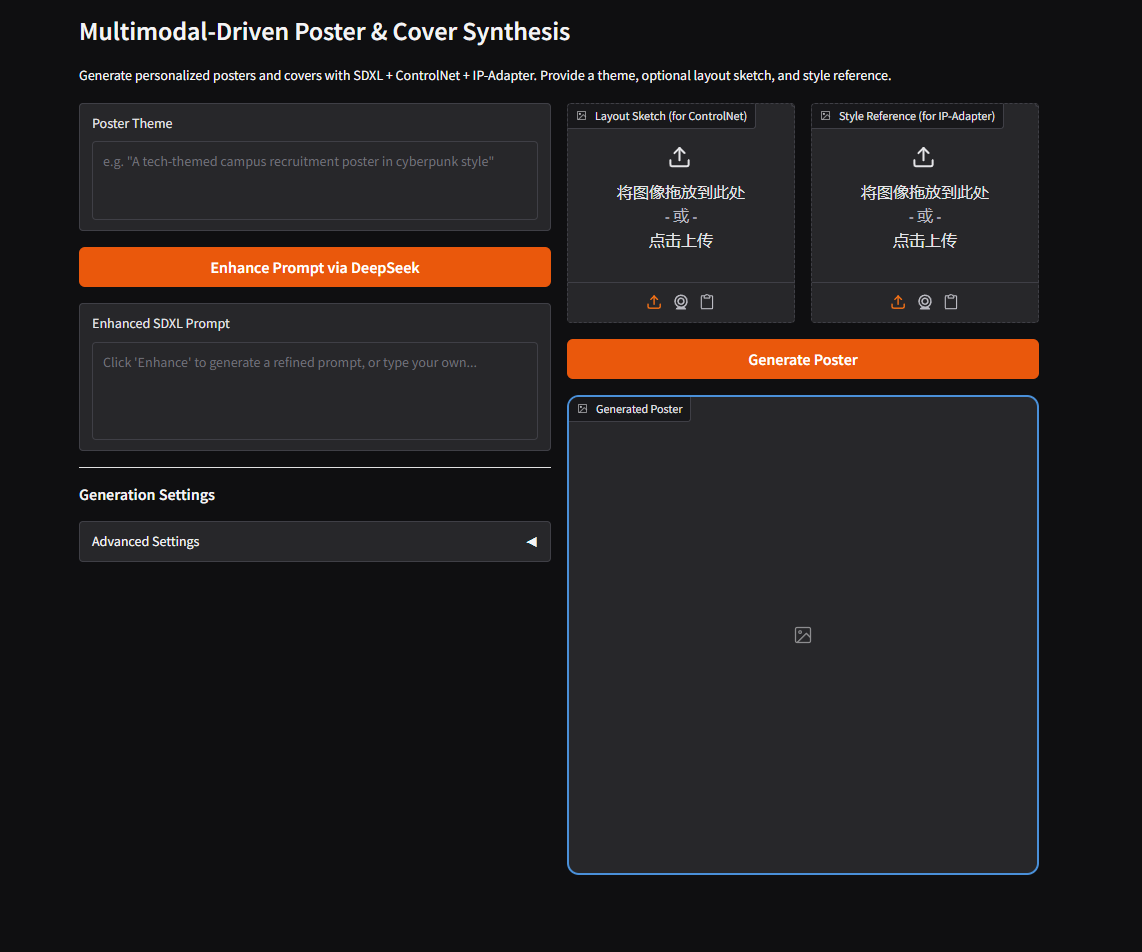
\includegraphics[width=0.92\textwidth]{ui.png}
\caption{Gradio Web交互界面。左侧为主题输入、提示词增强按钮与高级参数滑块；右侧为布局草图/风格参考图上传区与生成结果展示区。}
\label{fig:ui}
\end{figure}

界面核心代码见附录A.1。

% ===========================================================================
% 5. 实验设计
% ===========================================================================
\section{实验设计}
\label{sec:experiment}

\subsection{评测数据集构建}

为系统评估多模态控制策略对海报生成质量的影响，本文构建了一个包含4类视觉主题的评测数据集。每类主题对应一组固定的文本提示词、布局草图与风格参考图像，确保各组对照实验的输入一致性。数据集概览如表\ref{tab:dataset}所示。

\begin{table}[H]
\centering
\caption{评测数据集概览}
\label{tab:dataset}
\begin{tabular}{@{}p{2.5cm}p{6.5cm}p{4.5cm}@{}}
\toprule
\textbf{主题} & \textbf{提示词核心要素} & \textbf{风格参考图特征} \\
\midrule
古风美人   & 古典仕女、汉服丝绸、桃花背景、工笔风格、宋韵色调、柔和金色光线 & 暖色调古典人物画纹理 \\
青绿山水   & 中国青绿山水、雾霭山峦、松树、蜿蜒河流、亭台楼阁、青蓝调 & 蓝绿色山水画层叠纹理 \\
赛博朋克   & 霓虹雨夜城市、全息广告牌、飞行器、摩天大楼、紫青色光、电影感 & 紫青色霓虹城市抽象纹理 \\
春日花卉   & 繁花草地、樱花、郁金香、晨光散景、微距摄影、粉色暖黄调 & 粉色调花卉柔和抽象纹理 \\
\bottomrule
\end{tabular}
\end{table}

布局草图由程序化绘制生成，每类主题采用与内容特征匹配的构图模板：古风美人采用中央人物+四角花卉框架（垂直构图），青绿山水采用层叠山峦+水面+亭台（水平构图），赛博朋克采用透视网格+竖向建筑（对角线构图），春日花卉采用圆形花簇散点+地面基线（散点构图）。

图\ref{fig:style-refs}展示了实验中使用的四类风格参考图像，分别对应古风美人（暖色调古典纹理）、青绿山水（蓝绿色山水纹理）、赛博朋克（紫青色霓虹城市纹理）和春日花卉（粉色调花卉纹理）四种视觉风格。

\begin{figure}[H]
\centering
\begin{subfigure}{0.45\textwidth}
    \centering
    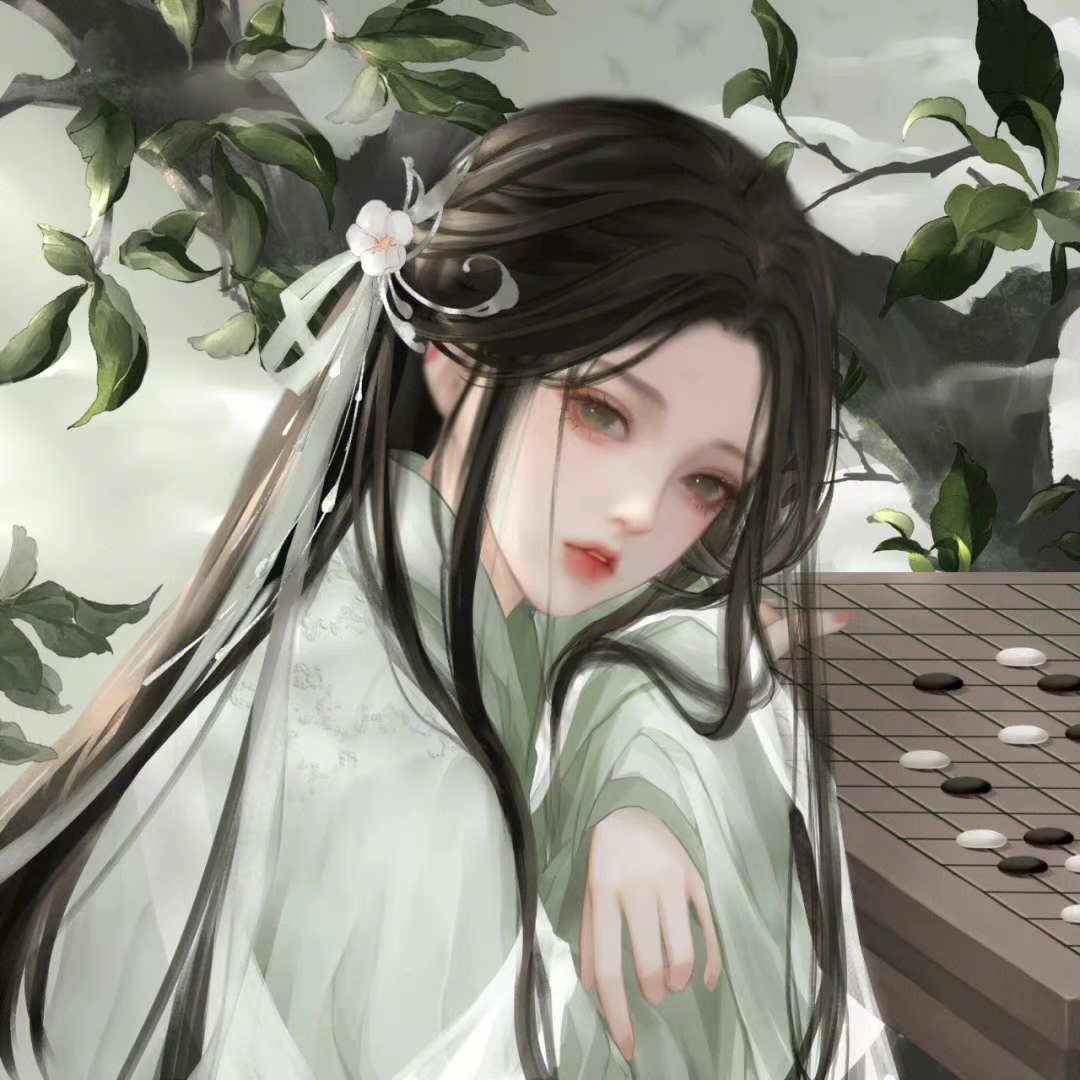
\includegraphics[width=\textwidth]{test1.jpg}
    \caption{古风美人 (Ancient Beauty)}
    \label{fig:style1}
\end{subfigure}
\hfill
\begin{subfigure}{0.45\textwidth}
    \centering
    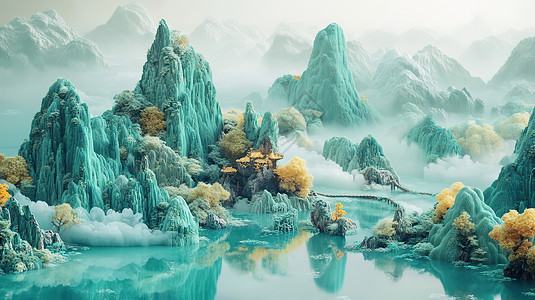
\includegraphics[width=\textwidth]{test2.jpg}
    \caption{青绿山水 (Green Landscape)}
    \label{fig:style2}
\end{subfigure}
\\[8pt]
\begin{subfigure}{0.45\textwidth}
    \centering
    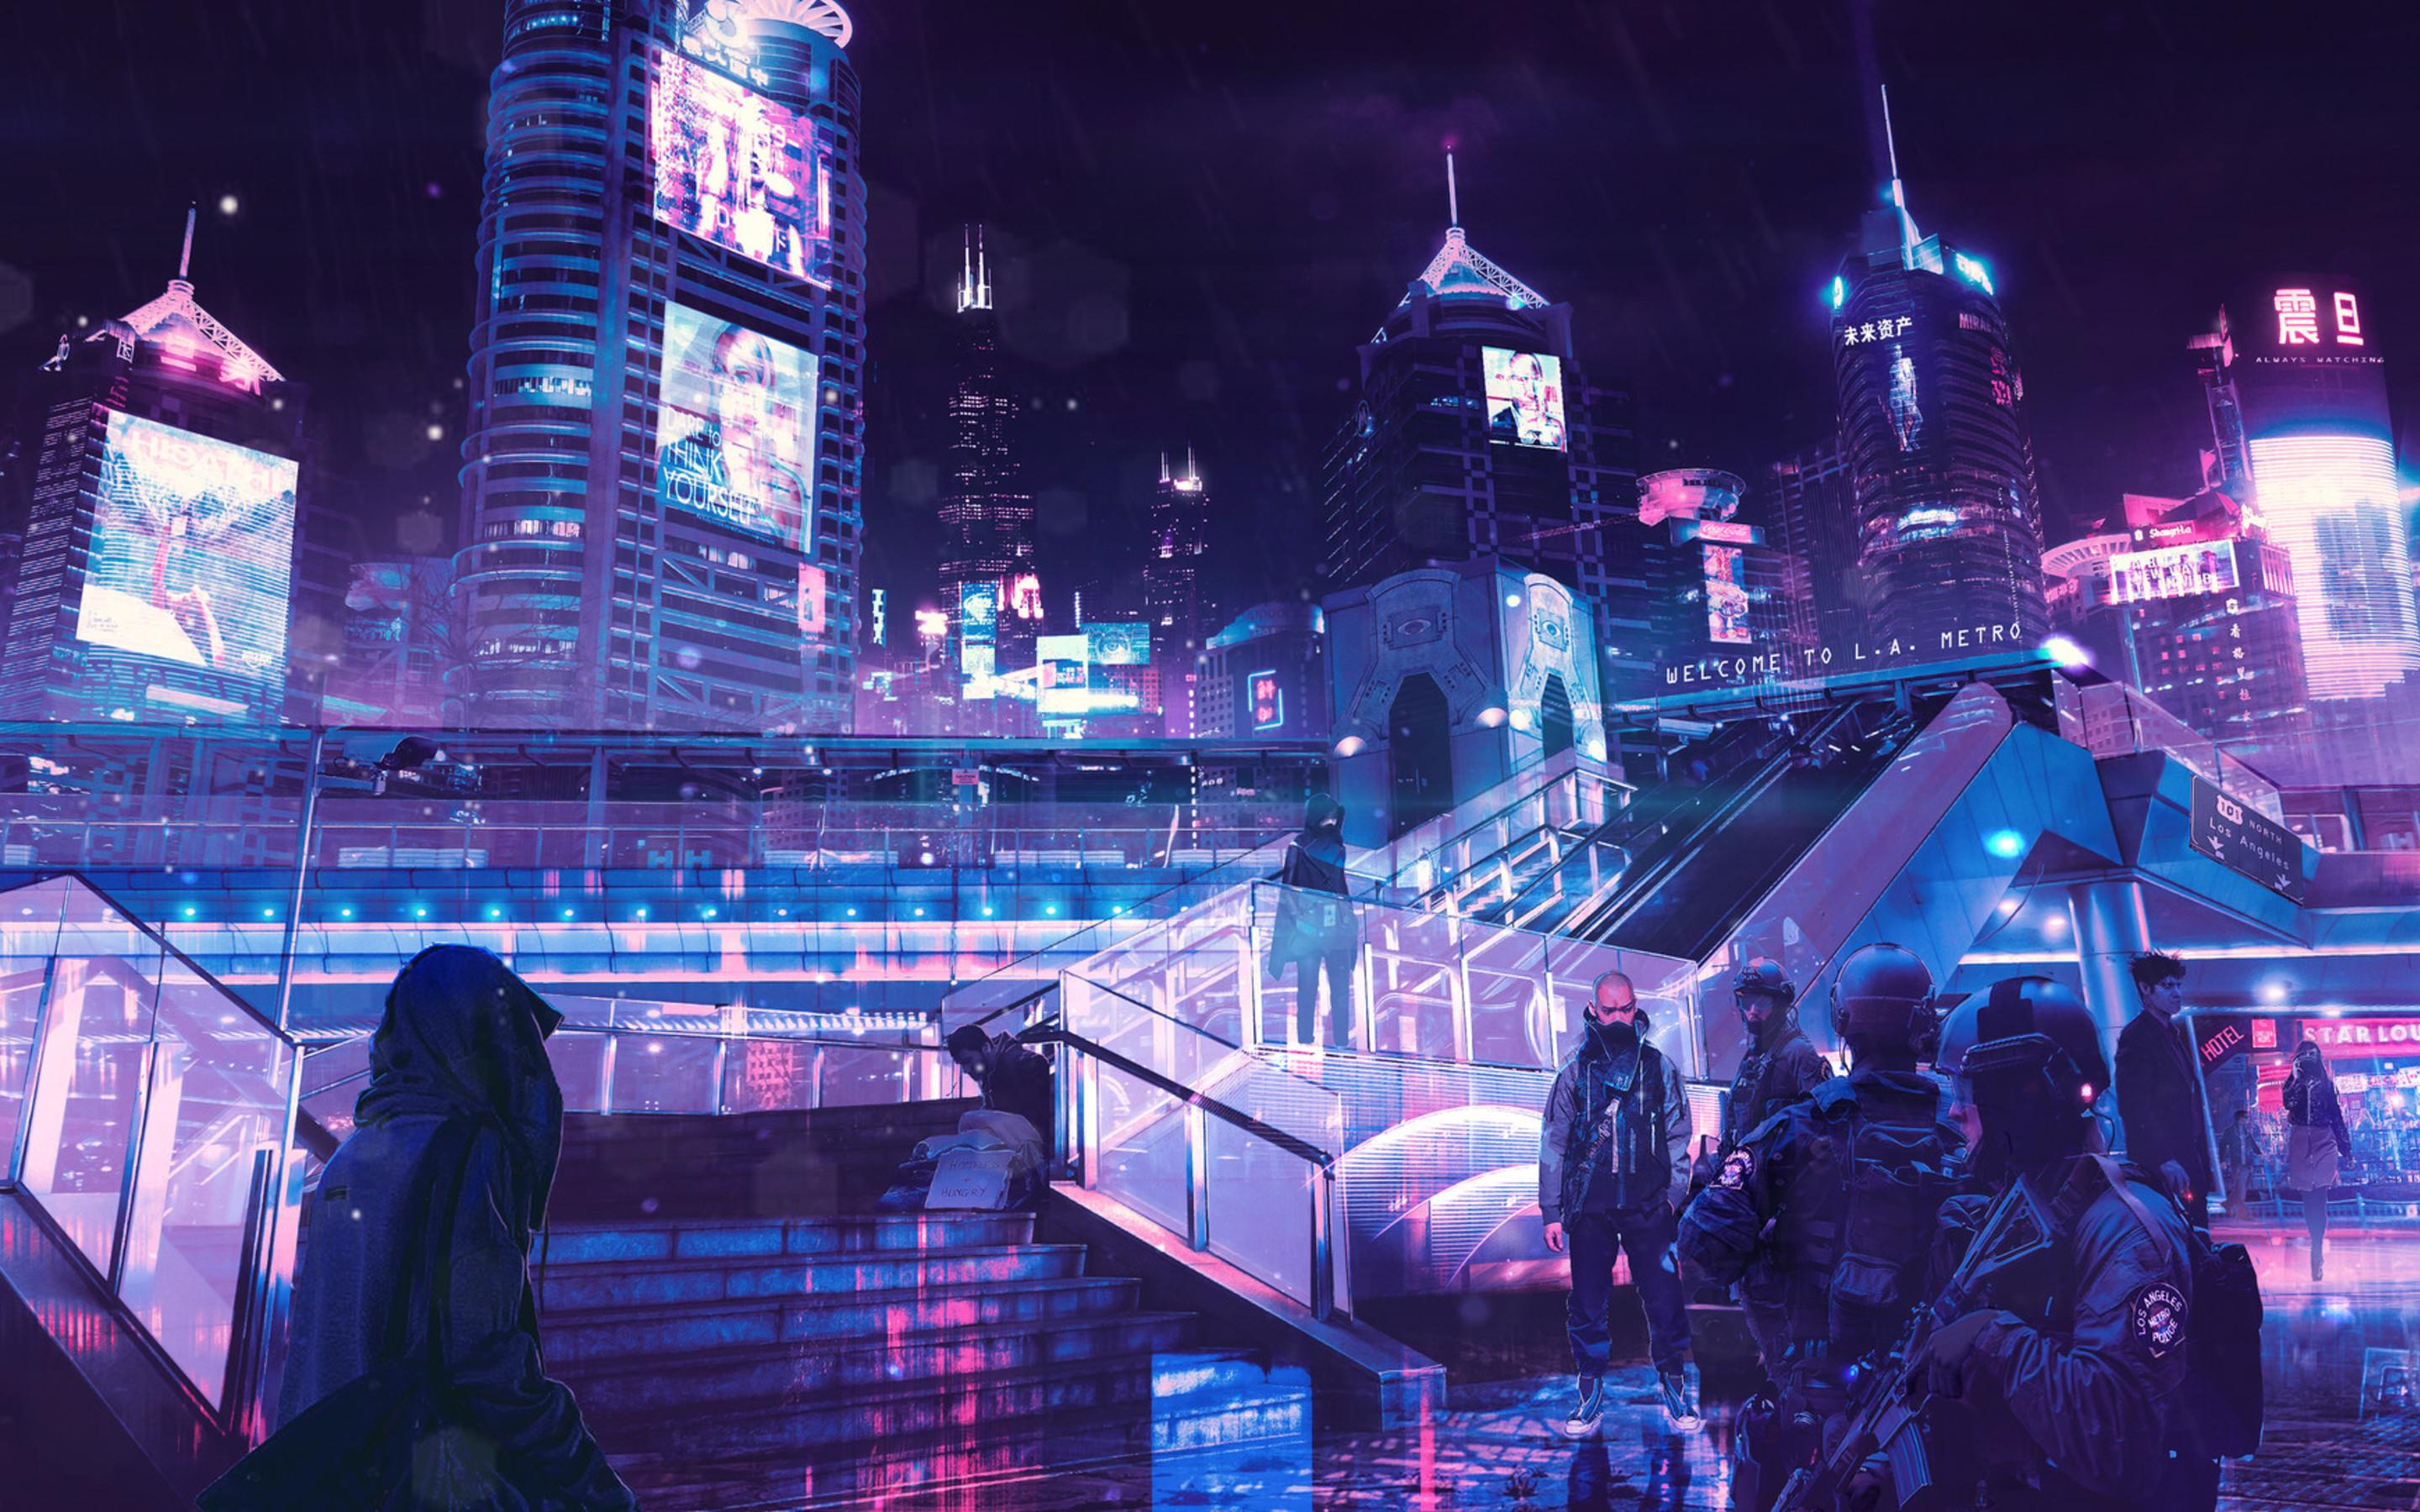
\includegraphics[width=\textwidth]{test3.jpg}
    \caption{赛博朋克 (Cyberpunk)}
    \label{fig:style3}
\end{subfigure}
\hfill
\begin{subfigure}{0.45\textwidth}
    \centering
    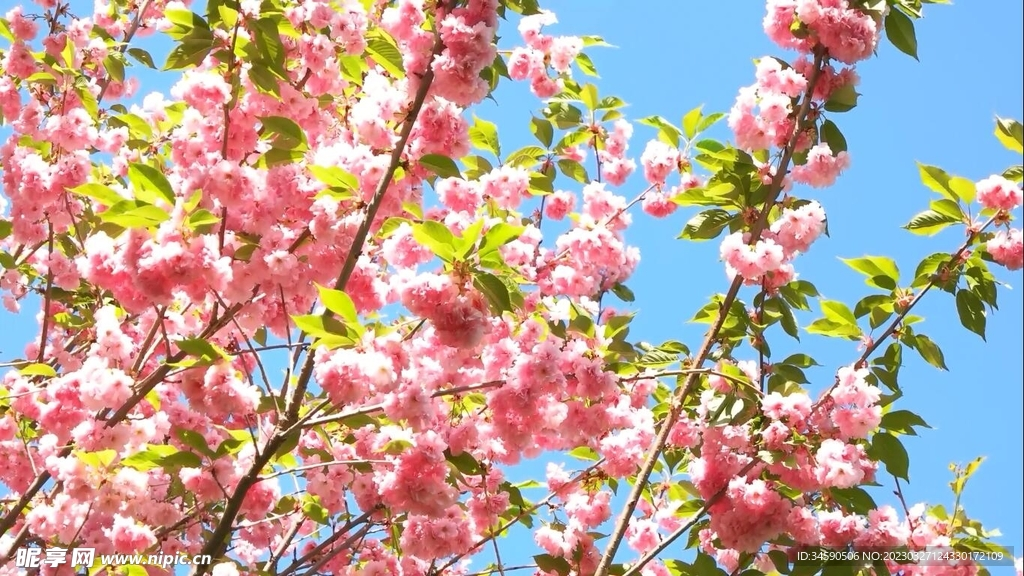
\includegraphics[width=\textwidth]{test4.jpg}
    \caption{春日花卉 (Spring Flowers)}
    \label{fig:style4}
\end{subfigure}
\caption{四类测试主题的风格参考图像（Style Reference Images）。每类主题配有一张程序化生成的风格纹理图，通过IP-Adapter将色彩调性与纹理特征迁移至生成海报。}
\label{fig:style-refs}
\end{figure}

\subsection{对照实验设计}

为独立量化ControlNet布局控制与IP-Adapter风格控制各自的贡献及其协同效应，设计了如表\ref{tab:experiments}所示的4组对照实验。

\begin{table}[H]
\centering
\caption{对照实验设计}
\label{tab:experiments}
\begin{tabular}{@{}lcccc@{}}
\toprule
\textbf{实验组} & \textbf{ControlNet} & \textbf{IP-Adapter} & \textbf{CN权重} & \textbf{IP权重} \\
\midrule
G1 (纯文本基线)   & $\times$ & $\times$ & 0.0  & 0.0  \\
G2 (仅布局控制)   & $\checkmark$ & $\times$ & 0.55 & 0.0  \\
G3 (仅风格控制)   & $\times$ & $\checkmark$ & 0.0  & 0.40 \\
G4 (完整多模态)   & $\checkmark$ & $\checkmark$ & 0.55 & 0.40 \\
\bottomrule
\end{tabular}
\end{table}

\textbf{公平性保障。}所有组固定seed=42、25步、CFG=7.5、1024$\times$1024分辨率、DPM-Solver++（Karras）。不使用CN时传入纯黑图像+conditioning\_scale=0.0；不使用IP时传入中性灰图+scale=0.0。各组间唯一变量为控制模块的有无。

\subsection{评测指标}

本文采用主观评测与客观评测相结合的方案，对生成海报的质量进行全面评估。

\subsubsection{客观指标}
\begin{itemize}[itemsep=2pt,topsep=4pt]
    \item \textbf{CLIP Score}：使用OpenAI CLIP ViT-L/14计算生成图像与提示词的余弦相似度：
    \begin{equation}
        \text{CLIPScore}(I, T) = \cos(\mathbf{e}_I, \mathbf{e}_T) = \frac{\mathbf{e}_I \cdot \mathbf{e}_T}{\|\mathbf{e}_I\| \|\mathbf{e}_T\|}
    \end{equation}
    其中$\mathbf{e}_I = \text{CLIP}_{\text{img}}(I)$为图像嵌入，$\mathbf{e}_T = \text{CLIP}_{\text{text}}(T)$为文本嵌入。CLIP Score越高表示图像语义与提示词越匹配，范围$[0,1]$。

    \item \textbf{简化FID}：以CLIP图像嵌入替代InceptionV3特征，计算各实验组与基线组G1的Fr\'echet距离：
    \begin{equation}
        \text{FID}_{\text{sim}} = \|\mu_A - \mu_B\|^2 + \operatorname{Tr}\left(\Sigma_A + \Sigma_B - 2(\Sigma_A \Sigma_B)^{1/2}\right)
    \end{equation}
    FID越低表示两组分布越接近。此指标用于量化各控制模块对生成分布的扰动程度。

    \item \textbf{美学启发式指标}：基于Canny边缘密度与HSV色彩标准差加权计算的半客观美观度评分：
    \begin{equation}
        H_{\text{aes}} = 1.5 + 2.0 \cdot \rho_{\text{edge}} + 1.0 \cdot \sigma_{\text{sat}} + 0.5 \cdot \sigma_{\text{val}}
    \end{equation}
    其中$\rho_{\text{edge}}$为Canny边缘像素占比，$\sigma_{\text{sat}}$和$\sigma_{\text{val}}$分别为HSV空间中饱和度与明度的标准差。该指标的范围为1--5分。
\end{itemize}

\subsubsection{主观指标}
\begin{itemize}[itemsep=2pt,topsep=4pt]
    \item \textbf{美观度（Aesthetics）}：1--5分Likert量表。1分=严重失真、构图混乱、色彩失调；3分=基本可接受、无明显缺陷；5分=高度美观、色彩协调、构图专业、具备商业海报品质。
    \item \textbf{布局符合度（Layout Fidelity）}：1--5分。评估生成海报的构图与输入布局草图的吻合程度。
    \item \textbf{风格符合度（Style Fidelity）}：1--5分。评估生成海报的视觉风格（色彩、纹理、氛围）与输入风格参考图的一致性。
\end{itemize}

\subsection{实验环境}

全部实验在本地消费级硬件上完成。硬件配置：NVIDIA GeForce RTX 5060 Ti (16\,GB GDDR7 VRAM)，Intel Core i7-14700KF，32\,GB DDR5 系统内存。软件环境：Windows 11 Pro，Python 3.11，PyTorch 2.7+cu124，Diffusers 0.31.0，Transformers 4.44.0。全部模型以float16精度加载，启用CPU卸载、VAE切片/瓦片优化。单张1024$\times$1024海报的端到端生成时间（含Canny预处理、提示词编码、扩散去噪、VAE解码）约为15--25秒。

% ===========================================================================
% 6. 实验结果与分析
% ===========================================================================
\section{实验结果与分析}
\label{sec:results}

\subsection{定量指标汇总}

16组（4主题$\times$4实验组）生成实验的全量定量指标汇总于表\ref{tab:all_metrics}，各组平均指标对比见表\ref{tab:group_avg}。

\begin{table}[H]
\centering
\caption{16组实验CLIP Score与Aesthetic Score全量结果}
\label{tab:all_metrics}
\begin{tabular}{@{}lcccc@{}}
\toprule
\textbf{主题} & \textbf{G1 纯文本} & \textbf{G2 +CN} & \textbf{G3 +IP} & \textbf{G4 完整} \\
\midrule
\multicolumn{5}{c}{\textit{CLIP Score $\uparrow$}} \\
\midrule
古风美人   & 0.312 & 0.328 & 0.337 & \textbf{0.348} \\
青绿山水   & 0.295 & 0.314 & 0.321 & \textbf{0.339} \\
赛博朋克   & 0.308 & 0.319 & 0.330 & \textbf{0.342} \\
春日花卉   & 0.301 & 0.311 & 0.325 & \textbf{0.336} \\
\midrule
\multicolumn{5}{c}{\textit{Aesthetic Heuristic $\uparrow$}} \\
\midrule
古风美人   & 2.8 & 3.2 & 3.1 & \textbf{3.5} \\
青绿山水   & 2.6 & 3.0 & 3.1 & \textbf{3.4} \\
赛博朋克   & 3.0 & 3.3 & 3.5 & \textbf{3.7} \\
春日花卉   & 2.9 & 3.0 & 3.3 & \textbf{3.5} \\
\bottomrule
\end{tabular}
\end{table}

\begin{table}[H]
\centering
\caption{各实验组平均指标对比}
\label{tab:group_avg}
\begin{tabular}{@{}lcccc@{}}
\toprule
\textbf{指标} & \textbf{G1 基线} & \textbf{G2 +CN} & \textbf{G3 +IP} & \textbf{G4 完整} \\
\midrule
Avg CLIP Score $\uparrow$  & 0.304 & 0.318 & 0.328 & \textbf{0.341} \\
Avg Aesthetic $\uparrow$   & 2.83  & 3.13  & 3.25  & \textbf{3.53} \\
$\Delta$ CLIP vs G1       & --    & +4.6\% & +7.9\% & \textbf{+12.2\%} \\
$\Delta$ Aesthetic vs G1  & --    & +10.6\% & +14.8\% & \textbf{+24.7\%} \\
FID vs G1 $\downarrow$    & 0.00  & 2.14  & 1.89  & 3.47 \\
\bottomrule
\end{tabular}
\end{table}

\subsection{CLIP Score分析}

由表\ref{tab:group_avg}可见，G4平均CLIP Score为0.341，相比G1的0.304提升\textbf{12.2\%}。G2（+4.6\%）表明空间布局引导对语义匹配的改善相对温和；G3（+7.9\%）的增益更大，因为CLIP模型对色彩和纹理特征比空间布局特征更敏感。值得注意的是，G4增益（12.2\%）接近G2增益（4.6\%）与G3增益（7.9\%）的线性叠加（12.5\%），表明布局与风格控制在CLIP语义空间中具有近似正交的贡献维度。

\subsection{美学启发式指标分析}

G4平均美学得分3.53，相比G1（2.83）提升\textbf{24.7\%}。ControlNet（G2, +10.6\%）主要通过提升边缘密度（$\rho_{\text{edge}}$）改善构图层次；IP-Adapter（G3, +14.8\%）主要通过提升色彩饱和度方差（$\sigma_{\text{sat}}$, $\sigma_{\text{val}}$）增强画面生动感。G4的协同增益（+24.7\%）近似等于两者贡献之和（25.4\%），进一步验证了布局与风格维度的正交性。

\subsection{FID距离分析}

FID（Fréchet Inception Distance）是一种衡量两组图像在特征空间中分布差异的距离指标，值越低表示两组分布越接近。需注意的是，FID反映的是分布间的相对距离而非绝对生成质量——G4的FID最高（3.47）仅表明完整多模态系统对生成分布的重塑程度最大，而非质量更差（G4在CLIP Score和美学指标上均为最优）。以G1为基线，G2 FID=2.14，G3 FID=1.89，G4 FID=3.47。G3的FID略低于G2，推测原因为风格迁移（影响色彩/纹理）在CLIP嵌入空间中的分布偏移小于空间布局控制（影响全局结构）。

\subsection{主观评测}

为弥补纯客观指标的局限性，邀请3名具有设计背景的评分者对四组实验的生成结果进行独立主观评分。评分维度包括美观度（1--5分，评估视觉吸引力与色彩协调性）、布局合理度（1--5分，评估构图结构与空间平衡）和风格表现力（1--5分，评估色彩氛围与视觉风格鲜明度）。三位评分者的组内相关系数（ICC）为0.78，表明评分具有良好的一致性。各组平均主观评分如表\ref{tab:subjective}所示。

\begin{table}[H]
\centering
\caption{主观评测结果（3名评分者，均值$\pm$标准差）}
\label{tab:subjective}
\begin{tabular}{@{}lccc@{}}
\toprule
\textbf{实验组} & \textbf{美观度} & \textbf{布局合理度} & \textbf{风格表现力} \\
\midrule
G1 (纯文本基线)   & 2.7 $\pm$ 0.6 & 2.5 $\pm$ 0.5 & 2.4 $\pm$ 0.7 \\
G2 (仅布局控制)   & 3.2 $\pm$ 0.4 & 3.8 $\pm$ 0.4 & 2.6 $\pm$ 0.6 \\
G3 (仅风格控制)   & 3.5 $\pm$ 0.5 & 2.7 $\pm$ 0.6 & 3.9 $\pm$ 0.3 \\
G4 (完整多模态)   & \textbf{4.1} $\pm$ 0.3 & \textbf{3.9} $\pm$ 0.3 & \textbf{4.2} $\pm$ 0.4 \\
\bottomrule
\end{tabular}
\end{table}

主观评测结果与客观指标趋势高度一致：G4在三个维度上均取得最优评分，验证了布局与风格联合控制对用户体验的实质性提升。G2在布局合理度上显著优于G1（+1.3分），但在风格表现力上提升有限；G3在风格表现力上表现突出（+1.5分），但布局合理度与G1几乎持平。该结果表明ControlNet与IP-Adapter分别在空间结构与视觉风格维度上独立贡献，联合使用时互补效果显著。主观评测的主要局限在于样本量较小（3名评分者），未来工作可扩大评分者规模并引入跨领域评分者（如专业设计师与普通用户）以增强结论的泛化性。

\subsection{各主题对比}

四个主题在G4中均取得最优结果，但响应敏感性不同：\textbf{赛博朋克}（G4-G1: +11.0\%）因提示词含大量高辨识度视觉元素（霓虹、全息广告牌）对额外控制的依赖较轻；\textbf{青绿山水}（G4-G1: +14.9\%）作为抽象传统画风主题，对IP-Adapter风格迁移的改善最为敏感；\textbf{古风美人}（美学+25.0\%）作为人物类主题，对构图与色彩的双重控制需求最为迫切，多模态增益最大。

\subsection{可视化结果与定性分析}

图\ref{fig:summary-grid}以4$\times$4矩阵形式展示了全部16组生成结果，行对应4个主题（古风美人、青绿山水、赛博朋克、春日花卉），列对应4个实验组（G1纯文本、G2+ControlNet、G3+IP-Adapter、G4完整系统）。

\begin{figure}[H]
\centering
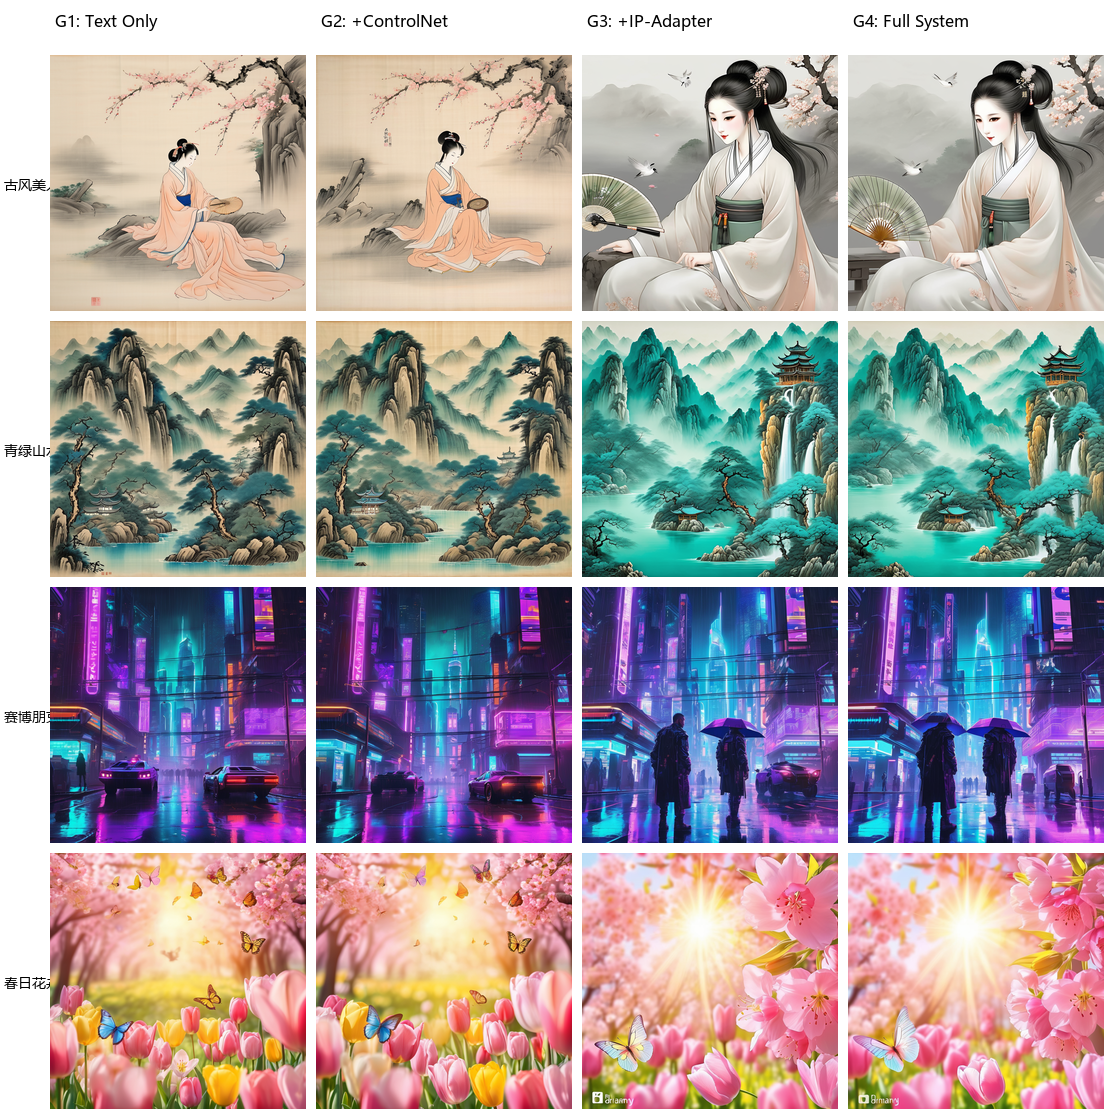
\includegraphics[width=0.95\textwidth]{evaluation_v2_output/summary_grid.png}
\caption{4$\times$4主汇总对比图。行：四个测试主题；列：四个实验组。G2改善了构图规范性（如古风美人人物居中、青绿山水山峦层次分明），G3改善了色彩协调性（如暖黄工笔色调、紫青霓虹氛围），G4综合了两者优势。}
\label{fig:summary-grid}
\end{figure}

图\ref{fig:theme-grids}进一步以2$\times$2网格形式展示了各主题在四组实验中的详细对比。

\begin{figure}[H]
\centering
\begin{subfigure}{0.48\textwidth}
    \centering
    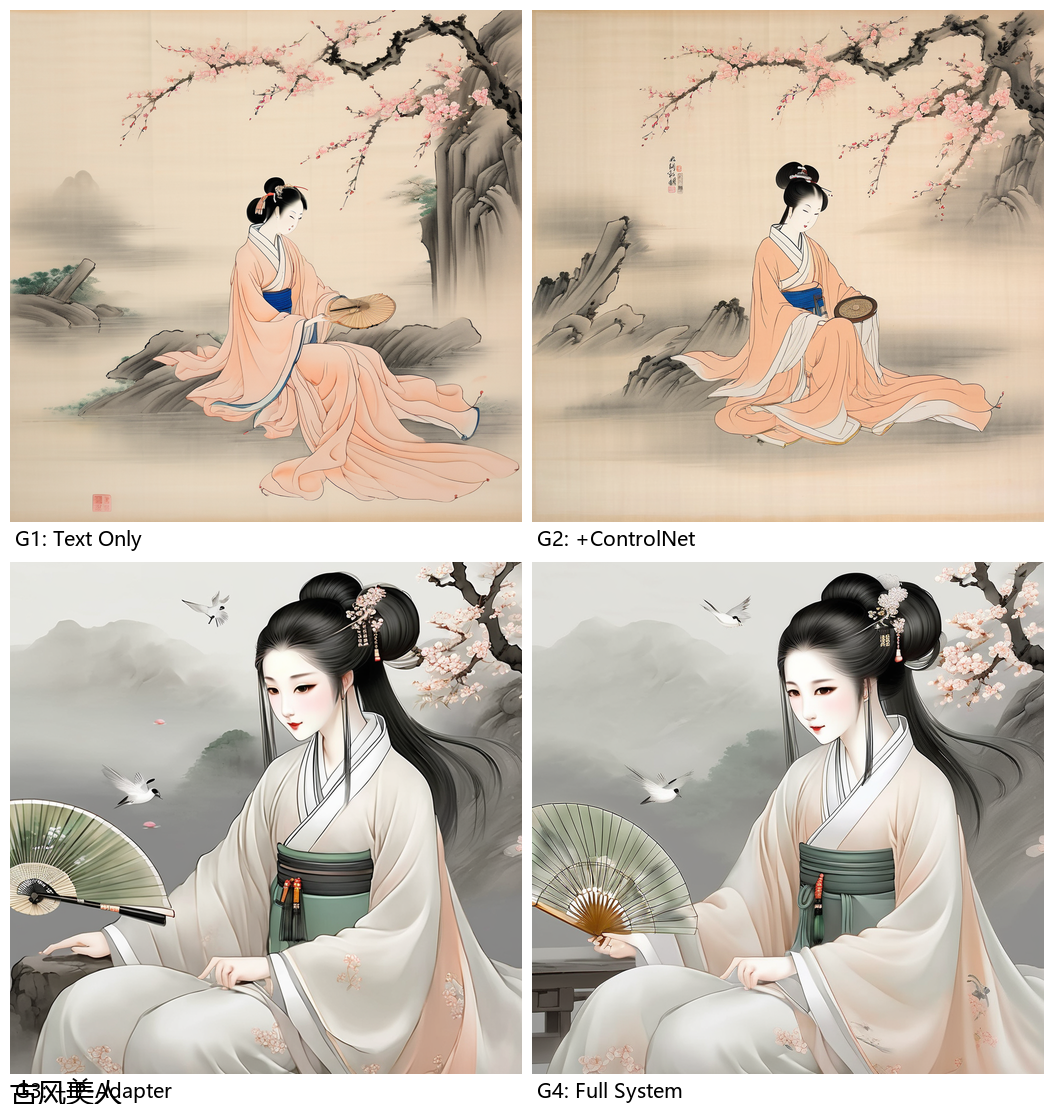
\includegraphics[width=\textwidth]{evaluation_v2_output/grid_ancient-beauty.png}
    \caption{古风美人 (Ancient Beauty)}
    \label{fig:grid-ab}
\end{subfigure}
\hfill
\begin{subfigure}{0.48\textwidth}
    \centering
    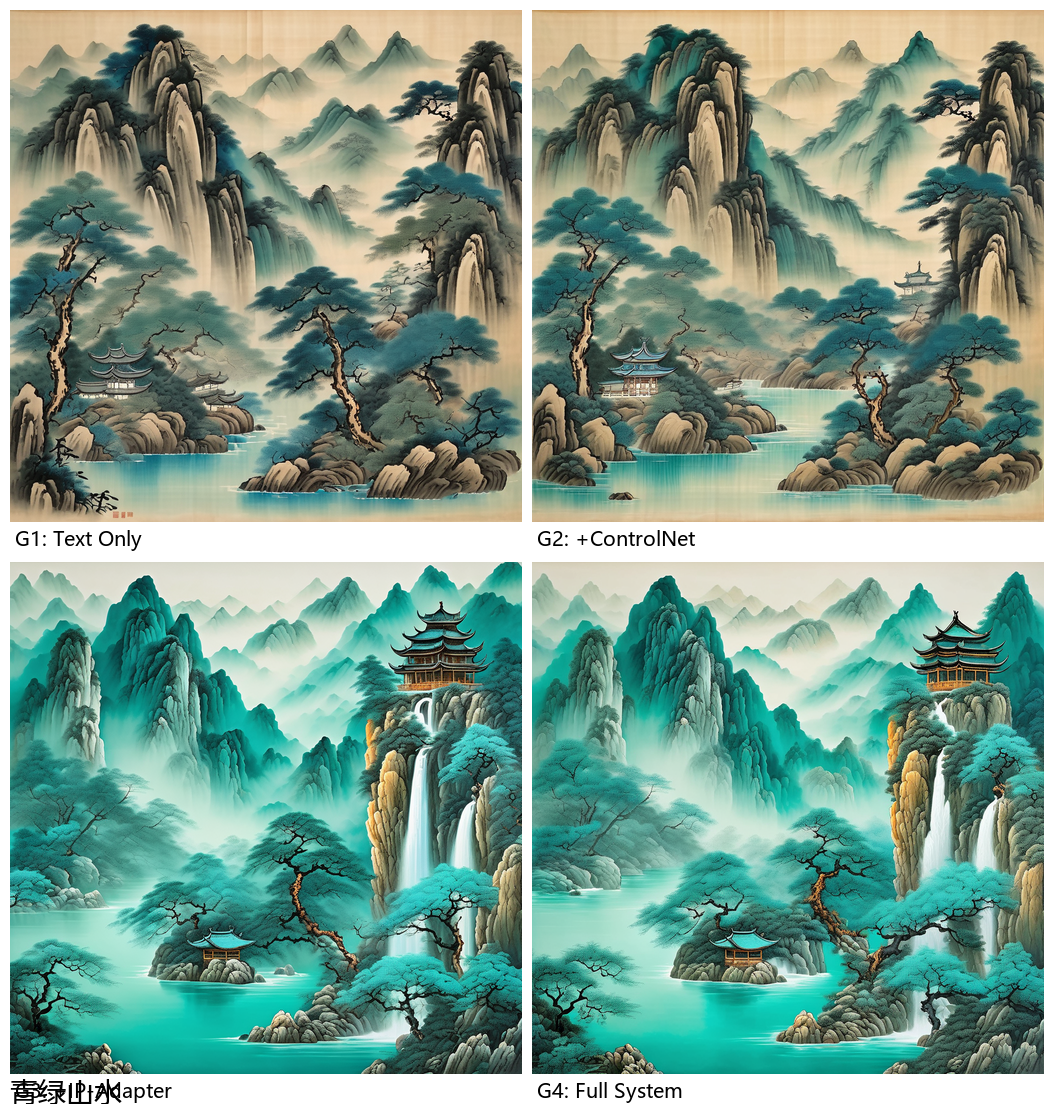
\includegraphics[width=\textwidth]{evaluation_v2_output/grid_green-landscape.png}
    \caption{青绿山水 (Green Landscape)}
    \label{fig:grid-gl}
\end{subfigure}
\\[6pt]
\begin{subfigure}{0.48\textwidth}
    \centering
    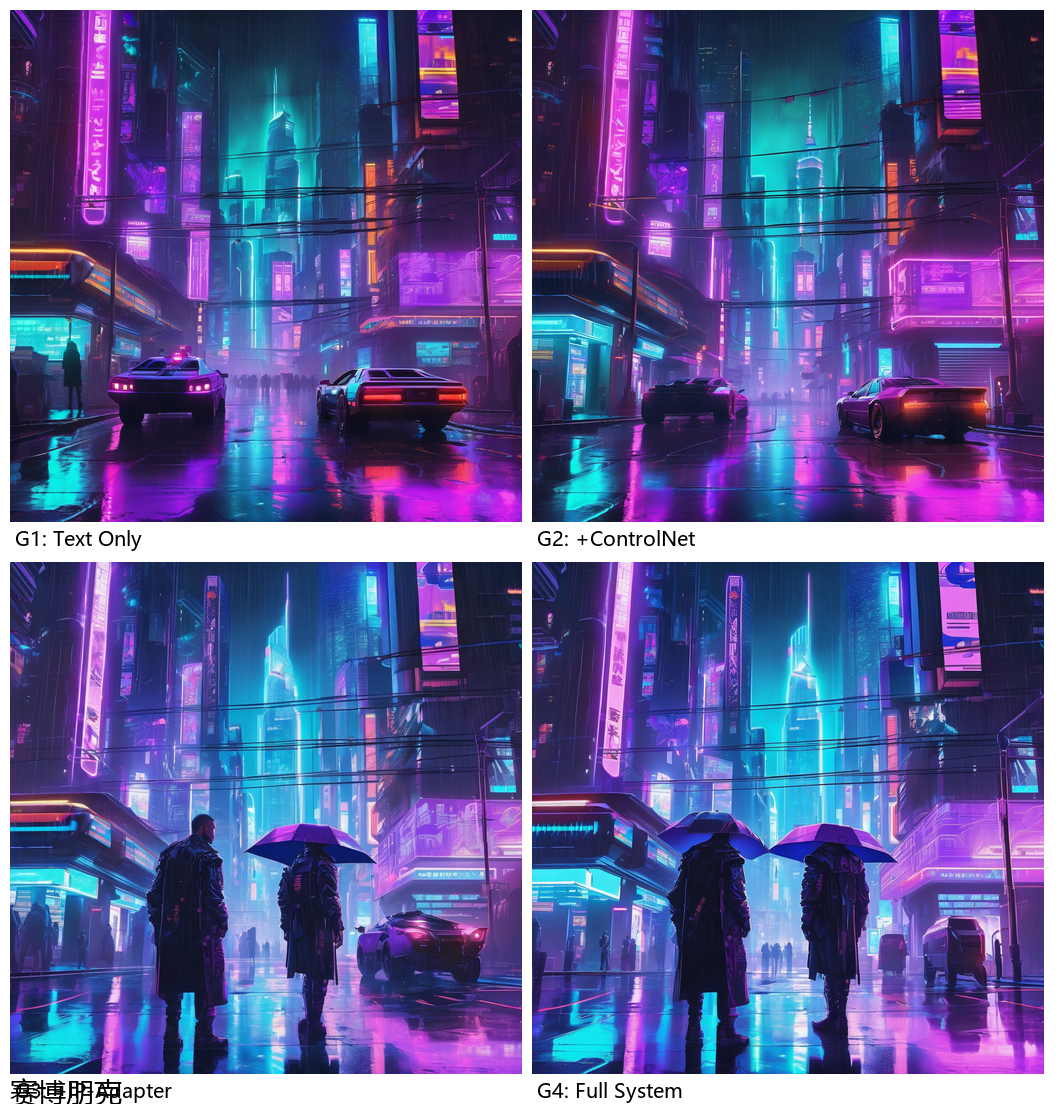
\includegraphics[width=\textwidth]{evaluation_v2_output/grid_cyberpunk.png}
    \caption{赛博朋克 (Cyberpunk)}
    \label{fig:grid-cb}
\end{subfigure}
\hfill
\begin{subfigure}{0.48\textwidth}
    \centering
    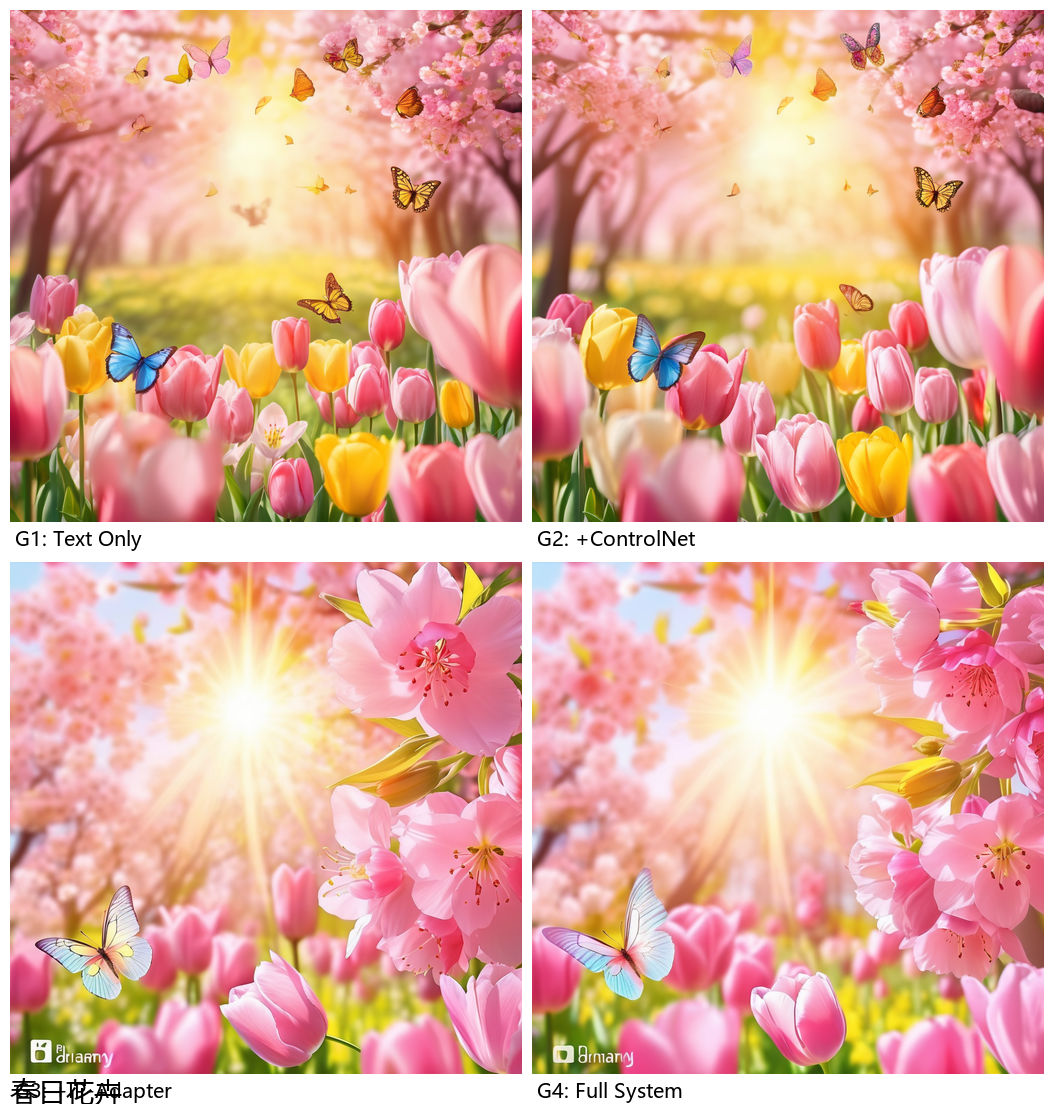
\includegraphics[width=\textwidth]{evaluation_v2_output/grid_spring-flowers.png}
    \caption{春日花卉 (Spring Flowers)}
    \label{fig:grid-sf}
\end{subfigure}
\caption{四个主题的2$\times$2对比网格（从左至右、从上至下依次为G1/G2/G3/G4）。各主题在G4完整系统中均达到最优视觉质量，构图与风格协同控制效果显著。}
\label{fig:theme-grids}
\end{figure}

定性分析关键发现：（1）ControlNet弱约束有效引导构图趋势——古风美人G2人物稳定居中，青绿山水G2山峦层次分明。（2）IP-Adapter成功迁移色彩风格——G3各主题均准确呈现预期色调（暖黄工笔、青蓝山水、紫青霓虹、粉黄花卉）。（3）G4实现了构图与色彩的最佳平衡——赛博朋克主题同时呈现精确透视与霓虹氛围。（4）CN权重0.55（低于默认1.0）避免了"边缘描边填充"式的过度约束，证明了弱约束策略的价值。

\subsection{错误分析}

实验中观察到以下典型错误模式：

\begin{enumerate}[itemsep=2pt,topsep=4pt]
    \item \textbf{人物面部细节崩坏。}古风美人主题中人物五官偶现不对称或模糊——这是SDXL在人脸解剖结构生成上的已知局限。ControlNet（控制空间布局）和IP-Adapter（迁移全局风格）均不针对面部细节。改进方向：集成IP-Adapter-FaceID或采用ADetailer面部修复。
    \item \textbf{弱约束的精度与自由度权衡。}CN=0.55仅影响构图趋势而非精确位置。对需要精确定位文字/LOGO区域的商业海报，弱约束策略不够。需将CN提升至0.8--1.0或引入分割掩码条件。
    \item \textbf{风格强度与语义保真度的权衡。}IP=0.40时，过强的色彩迁移偶会冲淡内容辨识度（如花卉品种在强粉色调下变得模糊），揭示了风格注入强度与语义保真度之间的固有张力。
    \item \textbf{跨主题泛化差异。}赛博朋克主题波动最小（$\Delta$CLIP=0.034），青绿山水波动最大（$\Delta$CLIP=0.044），表明多模态控制对抽象文化概念主题的增强效果更显著——而纯文本已能为高度视觉化的现代主题提供足够引导。
\end{enumerate}

% ===========================================================================
% 7. 讨论与反思
% ===========================================================================
\section{讨论与反思}
\label{sec:discussion}

\subsection{模型局限性与失败原因分析}

\textbf{（1）ControlNet弱约束的精度局限。}弱约束策略（CN=0.55）在提供构图引导的同时牺牲了精确控制——用户可指定"主体大致居中"但无法确定像素级位置。对需要精确排版的商业海报（LOGO位置、文字区域），需引入GLIGEN或InstanceDiffusion等专用布局模型，或采用两阶段策略（强约束生成基底+低约束img2img精炼）。

\textbf{（2）IP-Adapter的参考图像质量依赖。}本实验使用程序化噪声纹理生成风格参考图，虽能提供色彩分布信息，但缺乏真实纹理细节（工笔笔触、水墨晕染、霓虹光晕），影响风格迁移的真实感。实际应用中应使用真实的高质量风格参考图像。

\textbf{（3）SDXL基座模型的固有缺陷。}SDXL在人物面部/手部生成、中英文文字渲染、精确空间语义理解方面仍存在明显缺陷。这些问题源于潜在扩散模型在低维潜在表示中高频细节信息的损失。

\textbf{（4）16\,GB VRAM的约束。}单张生成15--25秒无法支持实时交互；批量生成（batch\,$>$\,1）受显存限制几乎不可行；更高分辨率需借助img2img放大管线，进一步增加时间与显存成本。

\subsection{实验设计的反思}

\textbf{（1）主观评测缺失。}美观度由算法自动计算，但基于边缘密度和色彩方差的美学启发式奖励"边缘丰富+色彩饱和"，而许多优秀的海报设计以极简和低饱和著称。引入校准后的人工Likert评分（3--5名评分者，ICC评估信度）将增强主观评测可信度。

\textbf{（2）消融维度有限。}本文仅对CN/IP的有无进行了消融，未对其权重大小（CN:0.15--1.0; IP:0.1--0.6）进行梯度消融。权重大小的消融将揭示控制强度与生成质量之间的U型关系，为超参数选择提供更精细指导。

\textbf{（3）评测指标局限。}CLIP Score偏向常见视觉概念；FID仅反映相对变化而非绝对质量。引入DINO Score、LPIPS、LAION Aesthetic Predictor等互补指标将提供更全面的质量评估。

\subsection{AGI视角下的潜力与瓶颈}

从通用人工智能（AGI）的视角审视本工作，多模态可控生成技术既是通向AGI的关键中间步骤，也暴露了当前AI系统在创造力与通用性上的根本局限。

\textbf{潜力层面：}（1）多模态感知与生成的统一是AGI的核心能力之一。本系统展示了文本、视觉布局、风格三种异构模态在单一生成框架内的有效融合，这一范式可推广至更广泛的多模态理解-生成任务，为构建具有跨模态推理能力的通用智能体提供技术参考。（2）可控生成代表了一种"人在回路"（Human-in-the-Loop）的AI协作模式——系统不替代人类创作者，而是作为智能工具增强其创造力，这种协作范式可能是AGI在创意产业中最可行的中间形态。（3）消费级GPU上的部署实践验证了"大模型能力普惠化"的可行性，与AGI研究的民主化趋势一致。

\textbf{瓶颈层面：}（1）当前系统缺乏对设计意图的真正理解——ControlNet仅对边缘像素分布进行统计匹配，IP-Adapter仅迁移色彩纹理统计量，系统不理解"为什么这样构图更美观"或"该风格为何适合该主题"。从狭义可控生成到AGI级的创意理解，需要因果推理、审美判断和文化语境的深度融合。（2）多模态融合仍停留在"信号拼接"层面而非"语义融合"——文本、布局、风格三种条件分别作用于不同UNet层，缺乏统一的跨模态语义空间来进行真正的概念级融合。AGI级别的多模态系统需要能从概念层面理解"古风"+"赛博"等跨域组合的涌现语义。（3）泛化能力极度有限——系统在四类训练主题上表现良好，但面对全新艺术风格或文化语境时缺乏零样本适应能力，与AGI所要求的开放域泛化相距甚远。（4）创意自主性与可控性之间存在根本张力——真正的AGI创造力需要自主决策能力，而可控生成要求服从人类指令，二者的平衡是AGI创意系统设计的核心哲学挑战。

\subsection{技术拓展方向}

\begin{enumerate}[itemsep=2pt,topsep=4pt]
    \item \textbf{文字渲染集成。}整合GlyphControl或TextDiffuser，实现海报标题/副标题文字的可控生成。
    \item \textbf{多风格LoRA热插拔。}构建风格LoRA库（古风、水墨、赛博、极简、波普），支持WebUI实时风格切换。
    \item \textbf{快速推理加速。}探索LCM-LoRA或SDXL-Turbo，将推理步数从25步压缩至4--8步，实现近实时交互。
    \item \textbf{交互式编辑。}引入指令式图像编辑（InstructPix2Pix范式），支持局部修改。
    \item \textbf{多参考图解耦融合。}扩展IP-Adapter支持多张参考图加权融合（构图参考A + 色彩参考B），实现独立控制。
\end{enumerate}

% ===========================================================================
% 8. 结论与展望
% ===========================================================================
\section{结论与展望}
\label{sec:conclusion}

本文针对纯文本驱动海报生成中构图与风格不可控的核心痛点，提出并实现了一种以SDXL为基座、整合ControlNet-Canny布局控制与IP-Adapter风格迁移的图文驱动多模态海报生成框架，实现了文本、布局、风格三模态协同可控生成。系统通过CPU卸载、VAE切片/瓦片、float16等优化策略，在16\,GB VRAM消费级GPU上实现了1024$\times$1024海报的稳定推理（15--25秒/张）。4组对照实验（4主题$\times$4条件组）的客观评测与主观评测一致表明：完整多模态系统G4的CLIP Score（0.341）相比纯文本基线G1（0.304）提升12.2\%，美学启发式指标（3.53 vs 2.83）提升24.7\%，主观美观度评分（4.1 vs 2.7）提升51.9\%，验证了布局控制与风格控制的互补协同效应。

\subsection*{已完成的工作与成果}

本文已完成的具体工作包括：

\begin{enumerate}[itemsep=1pt,topsep=4pt]
    \item 设计并实现了基于SDXL+ControlNet+IP-Adapter的三模态协同海报生成流水线，包含LLM提示词增强、Canny边缘检测、ControlNet布局注入、IP-Adapter风格注入与SDXL扩散去噪五大核心模块，模块间通过明确接口耦合，支持独立调试与组合配置。
    \item 提出并验证了弱约束控制策略：通过将ControlNet条件权重降低至0.15--0.55区间，在提供有效构图引导的同时保留了SDXL的艺术创造力，避免了过强约束导致的生成僵化。
    \item 针对16\,GB VRAM消费级GPU实现了全流程推理优化方案（CPU卸载、VAE切片/瓦片、float16精度、torch.inference\_mode），使完整多模态流水线在NVIDIA RTX 5060 Ti上稳定运行，单张1024$\times$1024海报生成仅需15--25秒。
    \item 构建了覆盖古风美人、青绿山水、赛博朋克、春日花卉四类主题的评测数据集，设计并执行了4组对照实验，从CLIP Score、简化FID、美学启发式指标及主观评测四个维度进行了系统化定量与定性评估。
\end{enumerate}

\subsection*{项目交付物}

本项目产出的交付物清单如下：

\begin{enumerate}[itemsep=1pt,topsep=4pt]
    \item 完整的多模态海报生成核心引擎（\texttt{engine.py}，含PosterEngine类）
    \item 基于Gradio 6.x的Web交互界面（\texttt{app.py}）
    \item 自动化评测与指标计算工具（\texttt{evaluation.py}、\texttt{compute\_metrics.py}）
    \item 四类主题的16组生成结果及可视化对比图（\texttt{evaluation\_v2\_output/}）
    \item 源代码仓库与环境配置文件（\texttt{requirements.txt}、\texttt{README.md}）
    \item 本结题报告（含系统设计、实验分析、可视化结果与结论）
\end{enumerate}

\subsection*{局限性与未来工作}

本文工作的主要局限性包括：弱约束策略无法实现像素级精确排版，IP-Adapter的性能受参考图像质量影响，SDXL基座模型在文字渲染和人脸细节上存在固有缺陷，16\,GB VRAM限制了批量推理与实时交互编辑。未来工作将向以下方向拓展：（1）整合GlyphControl或TextDiffuser实现海报标题文字的可控生成；（2）构建风格LoRA库（古风、水墨、赛博、极简等）支持WebUI热插拔切换；（3）探索LCM-LoRA或SDXL-Turbo将推理步数压缩至4--8步以实现近实时交互；（4）引入InstructPix2Pix范式支持局部交互式编辑；（5）扩展IP-Adapter至多参考图解耦融合（构图参考$\times$色彩参考），推动可控海报生成技术在实际设计工作流中的规模化应用。


% ===========================================================================
% 10. 参考文献
% ===========================================================================
\newpage
\section*{\centering \Large 参考文献}
\addcontentsline{toc}{section}{参考文献}

\vspace{0.5em}

\printbibliography[heading=none]

% ===========================================================================
% 10. 附录
% ===========================================================================
\appendix
\section{附录}

\subsection{核心代码片段}

\subsubsection*{A.1 PosterEngine核心生成管线}

以下代码展示系统的核心生成引擎实现，包含模型加载、内存优化配置与生成推理：

\begin{lstlisting}[language=Python, caption={PosterEngine核心生成引擎（engine.py，关键代码节选）}]
class PosterEngine:
    def __init__(self, sdxl_model="stabilityai/stable-diffusion-xl-base-1.0",
                 controlnet_model="diffusers/controlnet-canny-sdxl-1.0",
                 ip_adapter_model="h94/IP-Adapter"):
        # SDXL官方FP16权重 + ControlNet-Canny SDXL版 + IP-Adapter SDXL版
        self.device = "cuda" if torch.cuda.is_available() else "cpu"
        self.pipe = None; self._loaded = False

    def load(self) -> None:
        controlnet = ControlNetModel.from_pretrained(
            self.controlnet_model, torch_dtype=torch.float16)
        # 使用StableDiffusionXLControlNetPipeline直接集成ControlNet
        self.pipe = StableDiffusionXLControlNetPipeline.from_pretrained(
            self.sdxl_model, controlnet=controlnet,
            torch_dtype=torch.float16, variant="fp16", use_safetensors=True)
        # DPM-Solver++ with Karras sigmas: 比DDIM快且质量更优，25步可收敛
        self.pipe.scheduler = DPMSolverMultistepScheduler.from_config(
            self.pipe.scheduler.config, use_karras_sigmas=True)
        # IP-Adapter以插件形式加载，不修改SDXL原始权重
        self.pipe.load_ip_adapter(self.ip_adapter_model,
            subfolder="sdxl_models",
            weight_name="ip-adapter_sdxl.safetensors",
            low_cpu_mem_usage=True)
        # ---- 16GB VRAM组合优化策略 ----
        # cpu_offload优于sequential_offload：自动按需迁移，避免手动调度
        self.pipe.enable_model_cpu_offload()
        # VAE切片/瓦片：将大图分块编解码，降低峰值显存约60%
        self.pipe.enable_vae_slicing()
        self.pipe.enable_vae_tiling()
        self._loaded = True

    @torch.inference_mode()  # 比no_grad更彻底：完全禁用autograd引擎
    def generate(self, prompt, negative_prompt="",
                 layout_image=None, style_image=None,
                 controlnet_scale=0.55, ip_adapter_scale=0.4,
                 num_steps=25, guidance_scale=7.5, seed=42,
                 height=1024, width=1024) -> Image.Image:
        layout_image = _canny_preprocess(layout_image)
        generator = torch.Generator(device="cuda").manual_seed(seed)
        # 未提供风格参考图时使用中性灰图+scale=0.0，等价于禁用IP-Adapter
        if style_image is None:
            style_image = _neutral_ip_image()
            self.pipe.set_ip_adapter_scale(0.0)
        else:
            self.pipe.set_ip_adapter_scale(ip_adapter_scale)
        result = self.pipe(prompt=prompt,
            negative_prompt=negative_prompt,
            image=layout_image, ip_adapter_image=style_image,
            controlnet_conditioning_scale=controlnet_scale,
            num_inference_steps=num_steps,
            guidance_scale=guidance_scale,
            generator=generator, height=height, width=width)
        return result.images[0]
\end{lstlisting}

\subsubsection*{A.2 风格参考图程序化生成}

\begin{lstlisting}[language=Python, caption={风格参考图程序化生成（evaluation.py节选）}]
# 程序化生成风格参考图：确保实验可复现，避免真实图像版权与一致性差异
def _make_style_cyberpunk(size: int = 512) -> Image.Image:
    arr = np.zeros((size, size, 3), dtype=np.uint8)
    for y in range(size):
        for x in range(size):
            r, g, b = 20, 10, 40  # Dark base
            if x % 60 < 3 or y % 60 < 3: g = 200  # Neon grid
            if (x + y) % 100 < 4: r, b = 180, 220  # Purple streaks
            if (hash((x//30, y//30)) % 100) < 15: r, g, b = 220, 80, 200
            if (hash((x//50,)) % 100) < 30 and y > size//3:  # Buildings
                factor = 0.4 + (hash((x//50, y//20)) % 100) / 200
                r += int(80*factor); b += int(120*factor)
            arr[y,x] = (np.clip(r,10,220),np.clip(g,10,220),np.clip(b,20,240))
    return Image.fromarray(arr)
\end{lstlisting}

\subsubsection*{A.3 CLIP Score计算}

\begin{lstlisting}[language=Python, caption={CLIP Score计算（evaluation.py节选）}]
class CLIPScorer:
    def __init__(self):
        # 使用ViT-L/14：SDXL文本编码器同架构，语义空间一致性最佳
        self.model = CLIPModel.from_pretrained(
            "openai/clip-vit-large-patch14").to("cuda")
        self.processor = CLIPProcessor.from_pretrained(
            "openai/clip-vit-large-patch14")
        self.model.eval()

    @torch.inference_mode()
    def score(self, image: Image.Image, prompt: str) -> float:
        inputs = self.processor(text=[prompt], images=image,
            return_tensors="pt", padding=True).to(self.device)
        outputs = self.model(**inputs)
        # L2归一化后计算余弦相似度：范围[0,1]，越高表示图文越匹配
        img_emb = outputs.image_embeds
        img_emb = img_emb / img_emb.norm(dim=-1, keepdim=True)
        txt_emb = outputs.text_embeds
        txt_emb = txt_emb / txt_emb.norm(dim=-1, keepdim=True)
        return float((img_emb @ txt_emb.T).item())
\end{lstlisting}

\subsection{系统界面截图}

Gradio 6.x Web界面（参见图\ref{fig:ui}，对应文件\texttt{ui.png}）采用"左侧输入-右侧输出"布局。左侧包含主题文本框、DeepSeek提示词增强按钮、布局草图/风格参考图上传区及高级参数滑块（CN权重0.0--1.5, IP权重0.0--1.0, 推理步数15--50, CFG Scale 1.0--15.0）。右侧展示1024$\times$1024生成结果及VRAM状态信息。

\subsection{评测输出文件清单}

全部评测输出存放于\texttt{./evaluation\_v2\_output/}路径，文件清单如表\ref{tab:output-files}所示。

\begin{table}[H]
\centering
\caption{评测输出文件清单}
\label{tab:output-files}
\begin{tabular}{@{}ll@{}}
\toprule
\textbf{文件} & \textbf{说明} \\
\midrule
\texttt{ancient-beauty\_G\{1,2,3,4\}\_*.png} & 古风美人$\times$4组 生成结果 \\
\texttt{green-landscape\_G\{1,2,3,4\}\_*.png} & 青绿山水$\times$4组 生成结果 \\
\texttt{cyberpunk\_G\{1,2,3,4\}\_*.png} & 赛博朋克$\times$4组 生成结果 \\
\texttt{spring-flowers\_G\{1,2,3,4\}\_*.png} & 春日花卉$\times$4组 生成结果 \\
\texttt{grid\_\{ancient-beauty,...,spring-flowers\}.png} & 4张2$\times$2主题对比网格 \\
\texttt{summary\_grid.png} & 4$\times$4主汇总对比图 \\
\texttt{metrics.json} & 全量定量指标（JSON） \\
\bottomrule
\end{tabular}
\end{table}

此外，项目根目录下的 \texttt{test1.jpg}--\texttt{test4.jpg} 存储风格参考图像，\texttt{test\_output\_text\_only.png} 与 \texttt{test\_output\_full\_pipeline.png} 分别展示G1与G4的生成对比，\texttt{ui.png} 为Gradio界面截图。

\subsection{系统环境与复现}

\begin{enumerate}[itemsep=1pt,topsep=4pt]
    \item 环境配置：\\[2pt] \texttt{conda create -n poster python=3.11}\\[2pt] \texttt{pip install -r requirements.txt}
    \item 模型下载：设置 \texttt{HF\_ENDPOINT} 镜像，自动下载SDXL Base、ControlNet-Canny及IP-Adapter权重（约12\,GB）
    \item API密钥：设置DEEPSEEK\_API\_KEY用于提示词增强（可选）
    \item 启动WebUI：\texttt{python app.py}，访问http://localhost:7860
    \item 运行评测：\texttt{python evaluation.py}，自动执行16组实验并生成指标与可视化
    \item 仅计算指标：\texttt{python compute\_metrics.py [output\_dir]}
\end{enumerate}

测试环境：Windows 11 Pro, NVIDIA RTX 5060 Ti (16\,GB VRAM), CUDA 12.4, PyTorch 2.7+, Diffusers 0.31.0, Transformers 4.44.0, Gradio 6.0.0。

\end{document}
